%%%%%%%%%%%%%%%%%%%% book.tex %%%%%%%%%%%%%%%%%%%%%%%%%%%%%
%
% sample root file for the chapters of your "monograph"
%
% Use this file as a template for your own input.
%
%%%%%%%%%%%%%%%% Springer-Verlag %%%%%%%%%%%%%%%%%%%%%%%%%%


% RECOMMENDED %%%%%%%%%%%%%%%%%%%%%%%%%%%%%%%%%%%%%%%%%%%%%%%%%%%
\documentclass[graybox,envcountchap,sectrefs]{svmono}

% choose options for [] as required from the list
% in the Reference Guide

\usepackage{mathptmx}
\usepackage{helvet}
\usepackage{courier}
%
\usepackage{type1cm}         

\usepackage{makeidx}         % allows index generation
\usepackage{graphicx}        % standard LaTeX graphics tool
                             % when including figure files
\graphicspath{{Figures/}}
\usepackage{multicol}        % used for the two-column index
\usepackage[bottom]{footmisc}% places footnotes at page bottom

% see the list of further useful packages
% in the Reference Guide

\makeindex             % used for the subject index
                       % please use the style svind.ist with
                       % your makeindex program
    \addtolength{\oddsidemargin}{-1.25in}
 	\addtolength{\evensidemargin}{-1in}
	\addtolength{\textwidth}{2.5in}

	\addtolength{\topmargin}{0in}
	\addtolength{\textheight}{1.5in}
%%%%%%%%%%%%%%%%%%%%%%%%%%%%%%%%%%%%%%%%%%%%%%%%%%%%%%%%%%%%%%%%%%%%%

\begin{document}

\author{Shiing-shen Chern}
\title{Complex Manifolds without Potential Theory}
\subtitle{with an appendix on the geometry of characteristic classes}
\maketitle

\frontmatter%%%%%%%%%%%%%%%%%%%%%%%%%%%%%%%%%%%%%%%%%%%%%%%%%%%%%%
\newcommand{\N}{\mathbb{N}}
\newcommand{\R}{\mathbb{R}}
\newcommand{\Q}{\mathbb{Q}}
\newcommand{\Z}{\mathbb{Z}}

\newcommand{\C}{\mathbf{C}}
\newcommand{\PP}{\mathbf{P}}
\newcommand{\HHH}{\mathbf{H}}
\newcommand{\DD}{\mathbf{D}}

\newcommand{\OO}{\mathcal{O}}
\newcommand{\B}{\mathcal{B}}
\newcommand{\cU}{\mathcal{U}}
\newcommand{\F}{\mathcal{F}}



\newcommand{\rO}{\mathrm{O}}
\newcommand{\op}{\mathrm{op}}
\newcommand{\rd}{~\mathrm{d}} %roman d
\newcommand{\GL}{\mathrm{GL}}
\newcommand{\SU}{\mathrm{SU}}
\newcommand{\SL}{\mathrm{SL}}
\newcommand{\SO}{\mathrm{SO}}
\newcommand{\U}{\mathrm{U}}
\newcommand{\Sp}{\mathrm{Sp}}
\newcommand{\im}{\mathrm{Im}}
\newcommand{\ord}{\mathrm{ord}}
\newcommand{\End}{\mathrm{End}}
\newcommand{\Aut}{\mathrm{Aut}}
\newcommand{\Hom}{\mathrm{Hom}}
\newcommand{\ad}{\mathrm{ad}}
\newcommand{\tr}{\mathrm{tr}}
\newcommand{\Rad}{\mathrm{Rad}}



% \newcommand{\DD}{\overline{\mathbf{D}}}


\newcommand{\res}{\mathsf{res}}



% %%%%%%%%%%%%%%%%%%%%%%% dedic.tex %%%%%%%%%%%%%%%%%%%%%%%%%%%%%%%%%
%
% sample dedication
%
% Use this file as a template for your own input.
%
%%%%%%%%%%%%%%%%%%%%%%%% Springer %%%%%%%%%%%%%%%%%%%%%%%%%%

\begin{dedication}
Use the template \emph{dedic.tex} together with the Springer document class SVMono for monograph-type books or SVMult for contributed volumes to style a quotation or a dedication\index{dedication} at the very beginning of your book in the Springer layout
\end{dedication}





% %%%%%%%%%%%%%%%%%%%%%%foreword.tex%%%%%%%%%%%%%%%%%%%%%%%%%%%%%%%%%
% sample foreword
%
% Use this file as a template for your own input.
%
%%%%%%%%%%%%%%%%%%%%%%%% Springer %%%%%%%%%%%%%%%%%%%%%%%%%%

\foreword

%% Please have the foreword written here
Use the template \textit{foreword.tex} together with the Springer document class SVMono (monograph-type books) or SVMult (edited books) to style your foreword\index{foreword} in the Springer layout. 

The foreword covers introductory remarks preceding the text of a book that are written by a \textit{person other than the author or editor} of the book. If applicable, the foreword precedes the preface which is written by the author or editor of the book.


\vspace{\baselineskip}
\begin{flushright}\noindent
Place, month year\hfill {\it Firstname  Surname}\\
\end{flushright}



%%%%%%%%%%%%%%%%%%%%%%preface.tex%%%%%%%%%%%%%%%%%%%%%%%%%%%%%%%%%%%%%%%%%
% sample preface
%
% Use this file as a template for your own input.
%
%%%%%%%%%%%%%%%%%%%%%%%% Springer %%%%%%%%%%%%%%%%%%%%%%%%%%

\preface

%% Please write your preface here
The main text, on complex manifolds, was the notes from a course with the same title given at UCLA in the fall of 1966. It was written up after each lecture; only minor change have been made. To the Department of Mathematics at UCLA, and Lowell Paige in particular, I wish to express here my belated thanks. The Appendix was an expanded version of a series of lectures given at a summer seminar of the Canadian Mathematical Congress taken place in Halifax, Nova Scotia in 1971. I wish to thank Professor J. R. Vastone for his hospitality and kindness. Noteworthy is the treatment of the secondary characteristic classes. which is different from the one given in the Bibliography to the Appendix.\par
Needless to say, my deepset gratitude is to the university of California at Berkeley and the National Science Foundation for their continuous support of my research.
 

% \vspace{\baselineskip}
% \begin{flushright}\noindent
% Place(s),\hfill {\it Firstname  Surname}\\
% month year\hfill {\it Firstname  Surname}\\
% \end{flushright}



% %%%%%%%%%%%%%%%%%%%%%%acknow.tex%%%%%%%%%%%%%%%%%%%%%%%%%%%%%%%%%%%%%%%%%
% sample acknowledgement chapter
%
% Use this file as a template for your own input.
%
%%%%%%%%%%%%%%%%%%%%%%%% Springer %%%%%%%%%%%%%%%%%%%%%%%%%%

\extrachap{Acknowledgements}

Use the template \emph{acknow.tex} together with the Springer document class SVMono (monograph-type books) or SVMult (edited books) if you prefer to set your acknowledgement section as a separate chapter instead of including it as last part of your preface.



\tableofcontents

% %%%%%%%%%%%%%%%%%%%%%%acronym.tex%%%%%%%%%%%%%%%%%%%%%%%%%%%%%%%%%%%%%%%%%
% sample list of acronyms
%
% Use this file as a template for your own input.
%
%%%%%%%%%%%%%%%%%%%%%%%% Springer %%%%%%%%%%%%%%%%%%%%%%%%%%

\extrachap{Acronyms}

Use the template \emph{acronym.tex} together with the Springer document class SVMono (monograph-type books) or SVMult (edited books) to style your list(s) of abbreviations or symbols in the Springer layout.

Lists of abbreviations\index{acronyms, list of}, symbols\index{symbols, list of} and the like are easily formatted with the help of the Springer-enhanced \verb|description| environment.

\begin{description}[CABR]
\item[ABC]{Spelled-out abbreviation and definition}
\item[BABI]{Spelled-out abbreviation and definition}
\item[CABR]{Spelled-out abbreviation and definition}
\end{description}


\mainmatter%%%%%%%%%%%%%%%%%%%%%%%%%%%%%%%%%%%%%%%%%%%%%%%%%%%%%%%
% %%%%%%%%%%%%%%%%%%%%%part.tex%%%%%%%%%%%%%%%%%%%%%%%%%%%%%%%%%%
% 
% sample part title
%
% Use this file as a template for your own input.
%
%%%%%%%%%%%%%%%%%%%%%%%% Springer %%%%%%%%%%%%%%%%%%%%%%%%%%

\begin{partbacktext}
\part{Part Title}
\noindent Use the template \emph{part.tex} together with the Springer document class SVMono (monograph-type books) or SVMult (edited books) to style your part title page and, if desired, a short introductory text (maximum one page) on its verso page in the Springer layout.

\end{partbacktext}
\chapter{Introduction and Examples}
A complex manifold is a paracompact Hausdorff space which has a covering by neighbourhoods each homeomorphic to an open set in the $m$-dimensional complex number space such that where two neighborhoods overlap the local coordinates transform by a complex analytic transformation. That is, if $z^1,\cdots,z^m$ are local coordinates in one such neighborhood and if $w^1,\cdots,w^m$ are local coordinates in another neighborhood, then where they are both defined, we have 
\[w^i=w^i(z^1,\cdots,z^m),\]
where each $w^i$ is a holomorphic (or analytic) function of the $z$'s and the functional determinant 
\[\frac{\partial (w^1,\cdots,w^m)}{\partial (z^1,\cdots,z^m)}\neq 0.\]
We will give some examples of complex manifolds:

\begin{example}
The complex number space $\C^m$ whose points are the ordered $m$-tuples of complex numbers $(z^1,\cdots,z^m)$. $\C^1$ is called the Gaussian plane.
\end{example}
\begin{example}
The complex projective space $\PP^m$. To define it, take $\C^{m+1}-0$, where $0$ is the point $(0,\cdots,0)$, and identify those points $(z^0,z^1,\cdots,z^m)$ which differ from each other by a factor. The resulting quotient space is $\PP^m$. It can be covered by $m+1$ open sets $U_i$ defined respectively by 
\[\{z^i\neq 0\}, \quad 0\leq i\leq m.\] 
In $U_i$ we have the local coordinates 
\[\zeta_i^k=\frac{z^k}{z^i},\quad 0\leq k\leq m,\ k\neq i.\]
The transition of local coordinates in $U_i\cap U_j$ is given by 
\[\zeta^h_j=\frac{\zeta^h_i}{\zeta^j_i}\quad 0\leq h\leq m,\ h\neq j,\]
which are holomorphic functions.\par
In particular, $\PP^1$ is the Riemann sphere.
\end{example}
% \include{Contents/ch2}
% %%%%%%%%%%%%%%%%%%%%% appendix.tex %%%%%%%%%%%%%%%%%%%%%%%%%%%%%%%%%
%
% sample appendix
%
% Use this file as a template for your own input.
%
%%%%%%%%%%%%%%%%%%%%%%%% Springer-Verlag %%%%%%%%%%%%%%%%%%%%%%%%%%

\appendix
\motto{All's well that ends well}
\chapter{Chapter Heading}
\label{introA} % Always give a unique label
% use \chaptermark{}
% to alter or adjust the chapter heading in the running head

Use the template \emph{appendix.tex} together with the Springer document class SVMono (monograph-type books) or SVMult (edited books) to style appendix of your book in the Springer layout.


\section{Section Heading}
\label{sec:A1}
% Always give a unique label
% and use \ref{<label>} for cross-references
% and \cite{<label>} for bibliographic references
% use \sectionmark{}
% to alter or adjust the section heading in the running head
Instead of simply listing headings of different levels we recommend to let every heading be followed by at least a short passage of text. Furtheron please use the \LaTeX\ automatism for all your cross-references and citations.


\subsection{Subsection Heading}
\label{sec:A2}
Instead of simply listing headings of different levels we recommend to let every heading be followed by at least a short passage of text. Furtheron please use the \LaTeX\ automatism for all your cross-references and citations as has already been described in Sect.~\ref{sec:A1}.

For multiline equations we recommend to use the \verb|eqnarray| environment.
\begin{eqnarray}
\vec{a}\times\vec{b}=\vec{c} \nonumber\\
\vec{a}\times\vec{b}=\vec{c}
\label{eq:A01}
\end{eqnarray}

\subsubsection{Subsubsection Heading}
Instead of simply listing headings of different levels we recommend to let every heading be followed by at least a short passage of text. Furtheron please use the \LaTeX\ automatism for all your cross-references and citations as has already been described in Sect.~\ref{sec:A2}.

Please note that the first line of text that follows a heading is not indented, whereas the first lines of all subsequent paragraphs are.

% For figures use
%
\begin{figure}[t]
\sidecaption[t]
%\centering
% Use the relevant command for your figure-insertion program
% to insert the figure file.
% For example, with the option graphics use
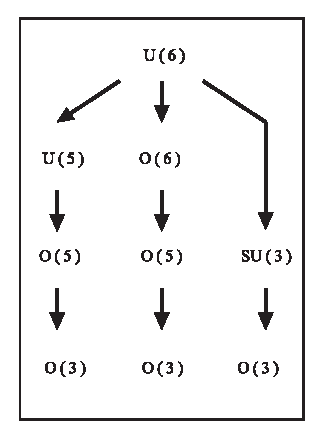
\includegraphics[scale=.65]{figure}
%
% If not, use
%\picplace{5cm}{2cm} % Give the correct figure height and width in cm
%
\caption{Please write your figure caption here}
\label{fig:A1}       % Give a unique label
\end{figure}

% For tables use
%
\begin{table}
\caption{Please write your table caption here}
\label{tab:A1}       % Give a unique label
%
% For LaTeX tables use
%
\begin{tabular}{p{2cm}p{2.4cm}p{2cm}p{4.9cm}}
\hline\noalign{\smallskip}
Classes & Subclass & Length & Action Mechanism  \\
\noalign{\smallskip}\hline\noalign{\smallskip}
Translation & mRNA$^a$  & 22 (19--25) & Translation repression, mRNA cleavage\\
Translation & mRNA cleavage & 21 & mRNA cleavage\\
Translation & mRNA  & 21--22 & mRNA cleavage\\
Translation & mRNA  & 24--26 & Histone and DNA Modification\\
\noalign{\smallskip}\hline\noalign{\smallskip}
\end{tabular}
$^a$ Table foot note (with superscript)
\end{table}
%


\backmatter%%%%%%%%%%%%%%%%%%%%%%%%%%%%%%%%%%%%%%%%%%%%%%%%%%%%%%%

% \Extrachap{Solutions}

\section*{Problems of Chapter~\ref{intro}}

\begin{sol}{prob1}
The solution\index{problems}\index{solutions} is revealed here.
\end{sol}


\begin{sol}{prob2}
\textbf{Problem Heading}\\
(a) The solution of first part is revealed here.\\
(b) The solution of second part is revealed here.
\end{sol}


% \printindex

%%%%%%%%%%%%%%%%%%%%%%%%%%%%%%%%%%%%%%%%%%%%%%%%%%%%%%%%%%%%%%%%%%%%%%

\end{document}





